\documentclass[12pt,a4paper]{article}
%Some packages I commonly use.
\usepackage{t1enc}
\usepackage[utf8]{inputenc} 
\usepackage[french]{babel}
\usepackage[titletoc]{appendix}
\usepackage[pdftex]{graphicx}
\usepackage{hyperref}
\usepackage{vmargin}
\usepackage{bbm}
\usepackage{graphicx}
\usepackage{caption}
\usepackage{subcaption}
\usepackage{tcolorbox}
\usepackage{framed}
\usepackage{amsmath}
\usepackage{amsthm}
\usepackage{amssymb}
\usepackage{amsfonts}
\usepackage{enumerate}
\usepackage{siunitx}
\usepackage{listingsutf8}
\usepackage{csquotes}
\usepackage[table]{xcolor}
\usepackage{mathtools, stmaryrd}
\usepackage[T1]{fontenc}
\usepackage{bookman}
\usepackage[utf8]{inputenc}
\usepackage[justification=centering]{caption}
\usepackage{multirow}
\usepackage{xspace}
\usepackage{xparse}
\DeclareMathOperator*{\argmax}{arg\!\max}
\DeclareMathOperator*{\argmin}{arg\!\min}
\setmargins{3cm}
{2cm} 
{15cm}
{22cm} 
{14pt}
{1cm}
{0pt} 
{1.5cm}
\pagestyle{plain} % pas d’en-tete, le pied de page contient le numéro de page centree
\setpapersize{A4}

\makeindex
\begin{document}
\begin{titlepage}
% -------------------------------------------------------------------
% You need to edit the details here
% -------------------------------------------------------------------
	\centering
	
\includegraphics[width=0.50\textwidth]{logo-sorbonne-universite-mise-en-avant.png}\par\vspace{1cm}
	\vspace{1cm}
	{\scshape\Large 3I005 : Statistique et Informatique\par}
	\vspace{1.5cm}
	{\large\huge Projet:\par}
	\vspace{0.5cm}
	{\large\huge\itshape  Exploration/Exploitation\par}
	\vspace{4cm}
	{\Large\itshape Par: \par  Angelo ORTIZ \par Celina HANOUTI\par}
	
	\vfill
	{\large Licence d'Informatique\par Ann\'ee 2018/2019\par}
\end{titlepage}

% -------------------------------------------------------------------
% Contents, list of figures, list of tables
% -------------------------------------------------------------------
\tableofcontents
\listoffigures
\listoftables
% -------------------------------------------------------------------
% Main sections (as required)
% -------------------------------------------------------------------
\newpage
\part*{Introduction}
\addcontentsline{toc}{part}{Introduction}

En intelligence artificielle, plus pr\'ecis\'ement en \textit{Machine Learning}, on est souvent amené, pour un ensemble de choix possibles, \`a trouver un bon compromis entre l’exploration et l'exploitation. L'exploration consiste à obtenir d'avantage d'informations dans le but de prendre de meilleures décisions dans le futur. L’exploitation, quant \`a elle, consiste \`a agir de manière optimale en fonction de ce qui est d\'ej\`a connu. Ce dilemme constitue un probl\`eme largement \'etudi\'e dans le domaine de l’apprentissage par renforcement. En effet, beaucoup d'algorithmes ont \'et\'e propos\'es pour r\'esoudre un certain nombre de ces probl\`emes.

\bigskip
Dans ce projet, nous allons \'etudier et analyser un certain nombre d'algorithmes basés sur le dilemme de {\itshape l’exploration vs exploitation} \`a travers des IAs de jeu. Dans un premier temps, nous allons effectuer une évaluation expérimentale d'algorithmes classiques dans un cadre simplifi\'e. La deuxi\`eme partie est consacr\'ee \`a l'implémentation d'un algorithme de Monte Carlo et enfin, dans les deux dernières parties, nous allons \'etudier des algorithmes plus avanc\'es ainsi qu'un jeu de strat\'egie combinatoire. 


\newpage
\part{Bandits-manchots}

\section{Description du probl\`eme}
On condi\`ere le probl\`eme d'apprentissage suivant : un agent est confront\'e \`a plusieurs reprises \`a un choix parmi N diff\'erentes actions, chacune des N actions procure une r\'ecompense moyenne $\mu^{i}$ inconnue par l'agent et nous d\'esignons l'action sélectionnée sur le pas de temps t par $a_{t}$, la r\'ecompense correspondante par $r_{t}$ et $N_{T}(a)$ le nombre de fois o\‘u l’action $a$ a \'et\'e choisi jusqu'au temps T.  L'objectif est de maximiser la somme des r\'ecompense obtenue au bout des $T$ premi\‘eres parties, pour cel\`a, l'agent doit identifier l'action au rendement le plus elev\'e $i^{*}$= $\argmax_{i \in {1,\ldots,N}}\mu^{i}$. Les valeurs $\mu^{i}$ etant inconnues, il est donc necessaire de faire des estimations qui doivent  \^etre le plus repr\'esentatives possible des valeurs $\mu^{i}$, notons $\hat{\mu}^{i}$ ces estimations. L'estimation associ\'ee \‘a une action est la r\'ecompense moyenne lorsque cette action est s\'electionn\'ee.
\begin{equation*}
\hat{\mu}^{i} = \frac{1}{N_{T}(a)}\sum_{t=1}^{T} r_{t}\mathbbm{1}_{a_{t} = a}
\end{equation*}

\section{Algorithmes}
Si de nombreux algorithmes ont \'et\'e propos\'es pour r\'esoudre ce dilemme, on se contentera ici d'en citer que quelques uns:
\subsection{Algorithme Al\'eatoire}
l'algorithme al\'eatoire se contente de choisir l’action uniform\'ement au hasard. On peut donc d\'ej\`a pr\'esager que cet algorithme sera forc\'ement le moins optimal.
{\bfseries En effet, il effectue purement de l'exploitation et est ainsi utilis\'e comme baseline pour les tests pr\'esent\'es par la suite}
\subsection{Algorithme Greedy}
L'algorithme Greedy est bas\'e sur une politique de selection tr\`es simple qui consiste \`a s\'electionner l'une des actions ayant la valeur estim\'ee la plus \'elev\'ee :
$a_{t}$ = $\argmax_{i \in {1,\ldots,N}}\hat{\mu}^{i}_{t}$.
Autrement dit, L'algorithme Greedy ne fait qu'\'exploiter les connaissances dont on dispose afin de maximiser la recompense \`a un instant $t$.
\subsection{Algorithme $\varepsilon$-Greedy}
Une approche courante pour trouver un compromis exploitation/exploration est l'algorithme $\varepsilon$-Greedy qui consiste \‘a choisir \‘a l’instant $t$, avec une probabilit\'e 1 - $\varepsilon$, l’action qui maximise le rendement moyen sur les estimations faites jusque l\‘a et avec une probabilit\‘e $\varepsilon$, une action uniform\‘ement au hasard. L'avantage de cet algorithme repose sur le fait que dans la mesure o\`u le nombre d'étape d'apprentissage augmente, chaque action sera choisie un nombre infini de fois assurant ainsi que tous les $\hat{\mu}^{i}$ convergeront vers les $\mu^{i}$. On peut conj\'ecturer la puissance de cet algorithme et sa capacit\'e \‘a explorer toutes les actions possibles et de prendre des d\'ecisions quasi proches de l’optimum.
{\bfseries Je sais pas si c'est vraiment un nombre infini, mais c'est s\^ur que les estimateurs se rapprocheront davantage aux gains moyens r\'eels. On pourra aussi dire que la valeur de $\varepsilon$ a un fort impact sur l'apprentissage, c'est pourquoi on en a test\'e diff\'erentes valeurs (constantes) et m\^eme une forme en fonction (d\'ecroissante) du temps ???}

\subsection{Algorithme UCB}
L'algorithme UCB est une autre strat\'egie qui permet de trouver une balance entre l'exploration et l'exploitation. L'id\'ee de cet algorithme consiste \`a se fier \`a une borne sup\'erieure de confiance, en effet, une incertitude existera toujours sur l'optimalit\'e des estimations faites jusque l\`a. Les deux algorithmes d\'efinis pr\'ecedemment choisissent toujours l'action qui semble meileure \`a un instant $t$ ou se contentent de choisir des actions al\'eatoirement sans distinction. L'algorithme UCB prend en compte l'optimalit\'e des estimations mais egalement l'incertitude sur celles-ci. Il selectionne l'action : $a_{t}$ = $\argmax_{i \in {1,\ldots,N}}(\hat{\mu}^{i}_{t} + \sqrt{\frac{2\log(t)}{N_{T}(i)}})$.
{\bfseries Ici, cette incertitude est mesur\'ee par le deuxi\`eme terme : plus grand est le d\'es\'equilibre entre le(s) (nombre d') actions effectu\'ees, plus on se m\'efie au r\'esultats. On privili\'egiera ainsi les actions le plus d\'efavoris\'ees}
\newpage
\section{Mise en oeuvre et analyse expérimentale}

\begin{figure}[htbp]
    \centering
    \begin{subfigure}[b]{0.47\textwidth} % "0.45" donne ici la largeur de l'image
        \centering 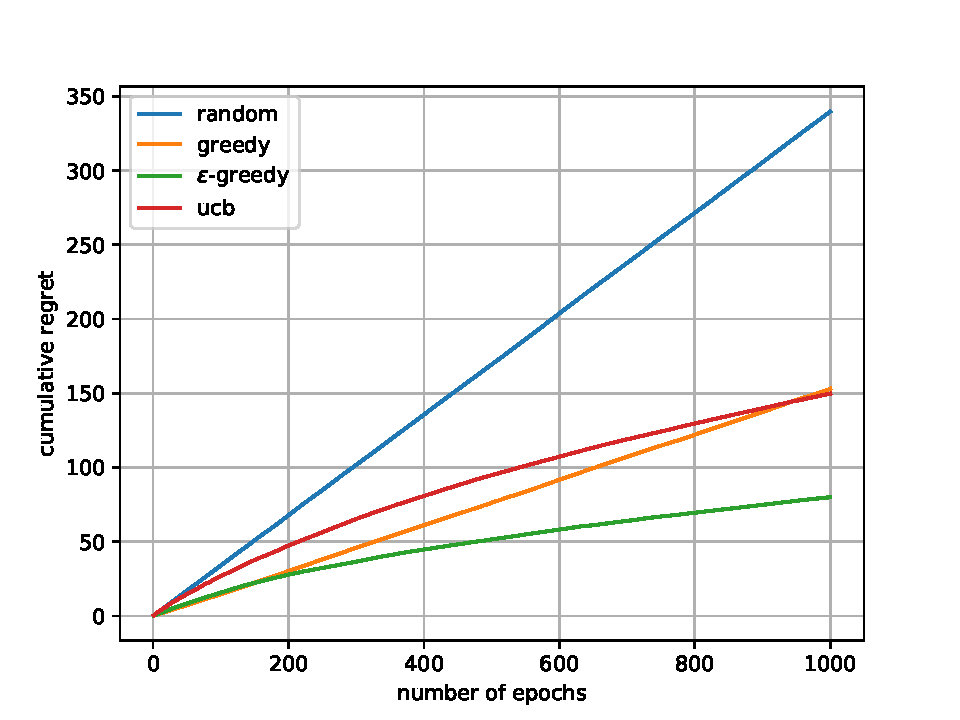
\includegraphics[width=\textwidth]{Report/sections/Figures/Figure1.pdf}
        \caption{Regret cumulé en fonction du nombre d'étape d'apprentissage}
    \end{subfigure}
    ~ 
    \begin{subfigure}[b]{0.47\textwidth}
        \centering 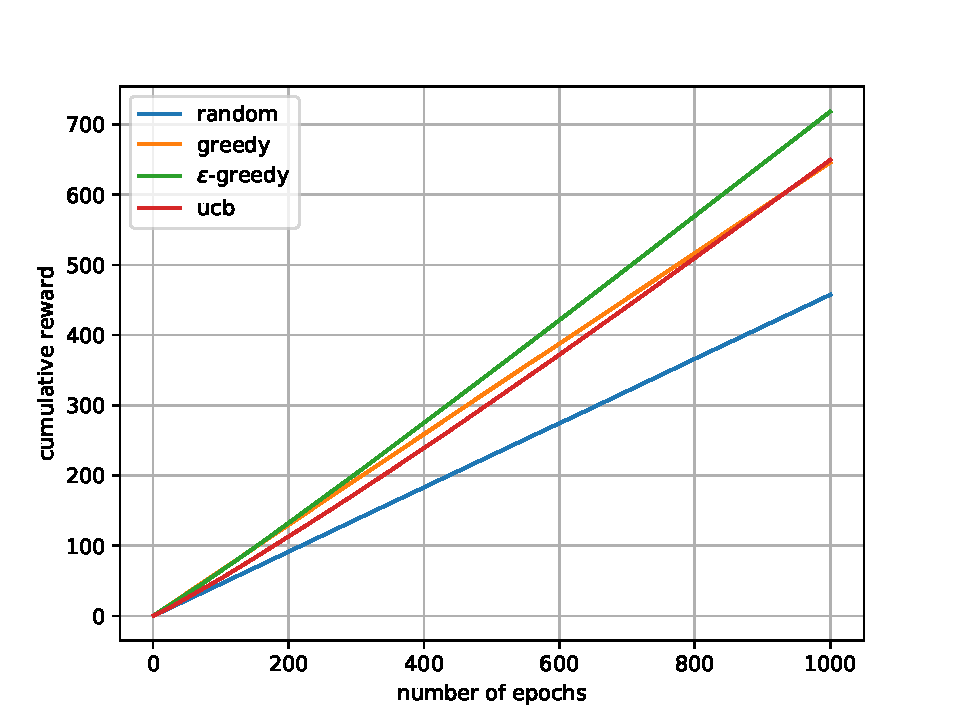
\includegraphics[width=\textwidth]{Report/sections/Figures/Figure2.pdf}
        \caption{Recompenses cumulés en fonction du nombre d'étape d'apprentissage}
    \end{subfigure}
    \caption{Performance des quatres algorithmes sur 10 leviers et en moyennant les résultats sur 400 éxecutions.}
\end{figure}
TODO : commenter les courbes ci-dessus. Il me semble qu'on est sensé remarquer une amelioration si on change la distribution de gain. En effet, si on a des gains qui suivent une distribution normale plutot qu'une distribution normale, on remarquera une legere amelioration des performance pour chaque algorithme. Cela est logique, car l'action optimale est mieux "s"paré" des autres actions (ici il serait plus judicieux de favoriser l'exploitation plutot que l'exploration)

\begin{figure}[htbp]
   \begin{subfigure}[b]{0.47\textwidth}
        \centering 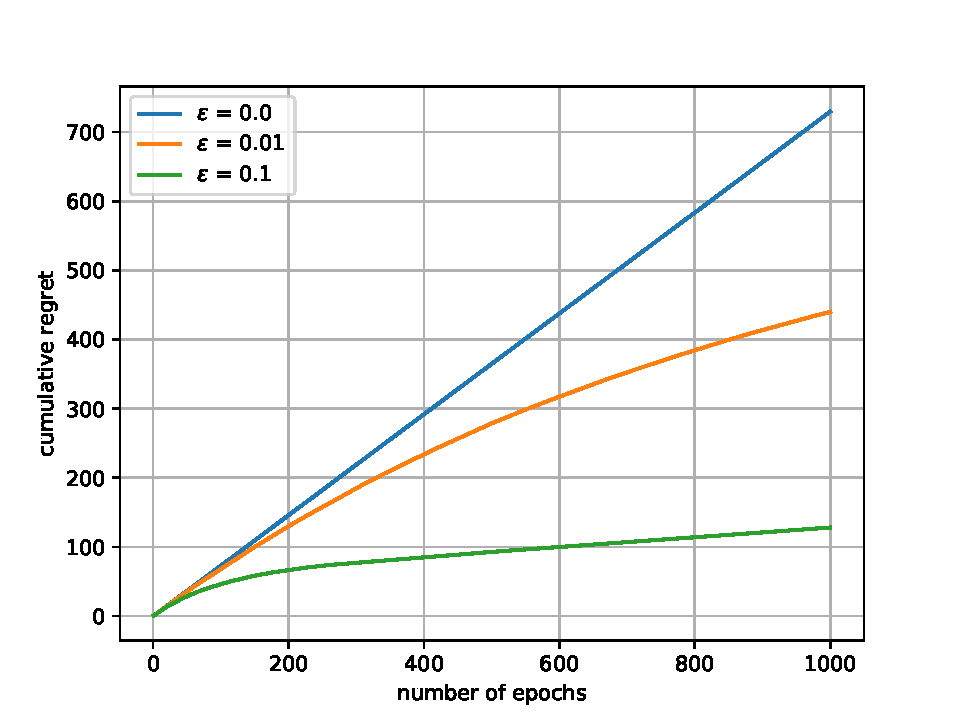
\includegraphics[width=\textwidth]{Report/sections/Figures/Figure3.pdf}
        \caption{Regret cumulé en fonction du nombre d'étape d'apprentissage}
    \end{subfigure}
    \begin{subfigure}[b]{0.47\textwidth}
        \centering 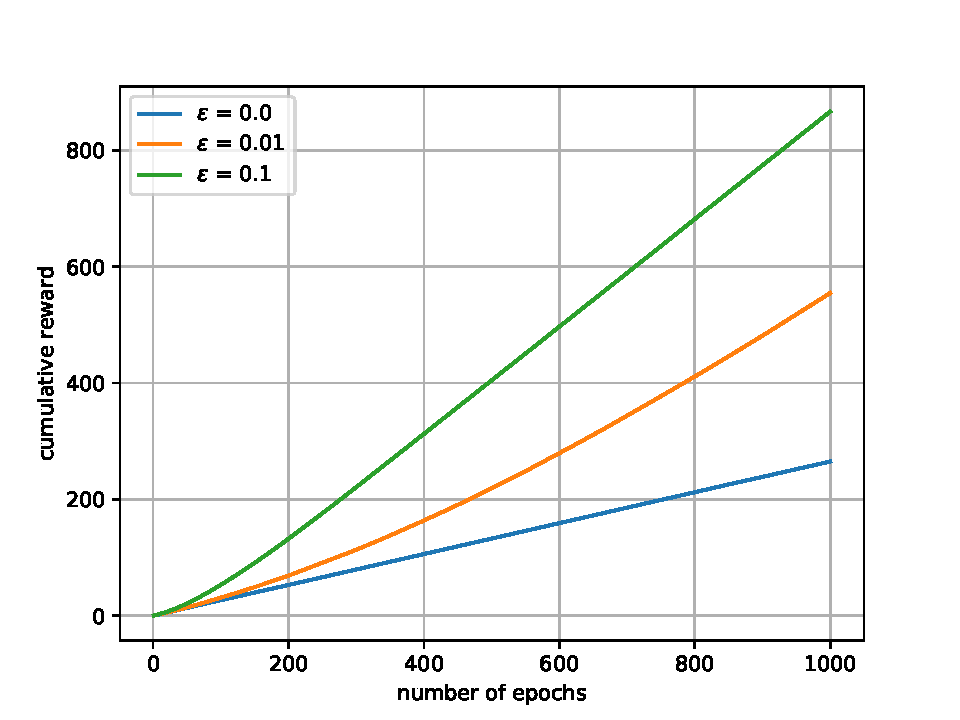
\includegraphics[width=\textwidth]{Report/sections/Figures/Figure4.pdf}
        \caption{Recompenses cumulés en fonction du nombre d'étape d'apprentissage}
    \end{subfigure}
    
    \caption{Performance des algorithmes Greedy et $\epsilon$-Greedy}
\end{figure}
La figure 2 illustre une comparaison entre la méthode $Greedy$ et deux autres méthodes $\epsilon$-$Greedy$ ($\epsilon$=0.01 et $\epsilon$=0.1). On remarque que le regret cumulé et le nombre de récompenses augmentent avec le nombre de pas d'apprentissage, on peut observer également qu'au tout début, l'algorithme $Greedy$ s'améliore en apprentissage au même rythme que les deux autres algorithmes puis on voit une diminution en performance. En effet, la méthode gloutonne effectue uniquement de l'exploitation, autrement dit, elle se contente de choisir l'action la plus prometteuse à un instant donné sans explorer d'autres actions qui pourrait l'être davantage, les echantillonages initiaux qu'elle a effectué sont avérés être sous optimaux par la suite ce qui explique son déclin de performance.
La méthode $\epsilon$-$Greedy$ avec $\epsilon$=0.1 a exploré bien plus que la méthode $\epsilon$=0.01 ce qui explique que la plupart du temps elle identifie l'action optimale assez rapidement. La méthode $\epsilon$-$Greedy$ avec $\epsilon$=0.01 s'améliore en apprentissage plus lentement car elle exploite plus mais à un moment donnée, on est sensé observer un gain de performance de tel sorte qu'elle donne de meilleurs résultats que $\epsilon$-$Greedy$ avec $\epsilon$=0.1.
\newline
#TODO: il serait intéressant de changer la dispersion des valeurs des récompenses, il me semble que si elles sont trop dispersées c'est à dire avec une variance non négligeable, il nous faudra plus d'exploration pour trouver l'action optimale et dans ce cas $\epsilon$-$Greedy$ sera plus pérformante que Greedy. mais si on a une variance assez faible, l'algorithme Greedy sera plus performant car il trouvera l'action optimale rapidement et ne fera plus d'exploration. à faire : courbe de l'evolution du pourcentage de gain afin qu'on puisse mieux observer le raisonnement précédent

\newpage
\part{Morpion et Monte Carlo}
\section{Description du problème}
Dans cette partie, on considère le célèbre jeu du Tic Tac Toe qui se joue sur une grille 3$\times$3. Les joueurs alternent tour à tour en plaçant un «X» ou un «O» sur une case vide de la grille. Le premier joueur à aligner trois symboles gagne. Nous allons considérer deux types de joueurs, des joueurs $Random$ qui se contenteront de choisir leurs prochains coups à jouer aléatoirement et des joueurs qui, eux, utiliseront une méthode de $Monte$ $Carlo$.  

\section{Joueur Aléatoire}
\begin{figure}[ht]
\centering
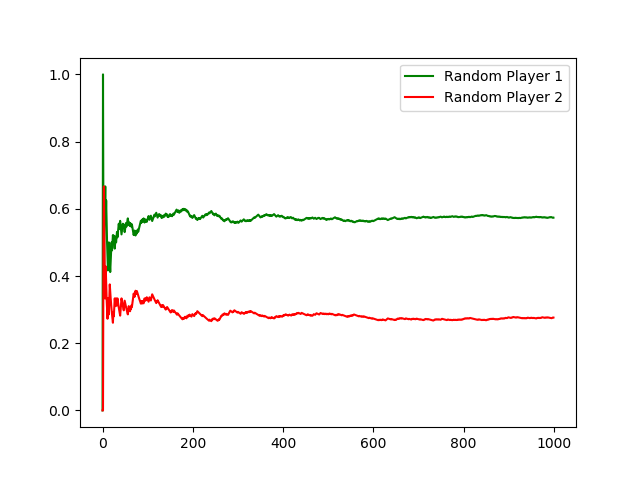
\includegraphics[width=0.6\textwidth]{Report/sections/Figures/Figure15.png}
\caption{Espérance de gain pour deux joueurs $Random$}
\label{FigGraphes}
\end{figure}
On considère une partie comme étant une expérience à deux issus : victoire ou défaite du Joueur 1.
On note $X$ la variable aléatoire qui dénote la victoire du Joueur 1, en cas de victoire, on donne à $X$ la valeur 1, sinon elle prend la valeur 0. Il est évident alors que $X$ suit une loi de Bernoulli, sur la figure ci-dessus, on peut déduire visuellement le paramètre $p$, en effet, en moyenne, le Joueur 1 a une probabilité
$\mathbb{P}$($X$=1)=0.6 de gagner. On en déduit que X suit une loi de Bernoulli de paramètre $p$=0.6 et de variance $\mathbb{V}$($X$)= $p$(1-$p$) = 0.24.

\section{Joueur Monte Carlo}
L'idée générale d'une simulation de $Monte$ $Carlo$ consiste à jouer un certain nombre de parties avec des choix aléatoires puis d'utiliser les résultats de ces parties pour calculer une bonne action à jouer. Lorsqu'un joueur gagne une de ces parties aléatoires, il devra privilégier les actions qui l'ont mené à cette victoire, dans l'espoir de choisir un coup gagnant lors des prochaines parties et éviter les actions qui ont mené son adversaire à la defaite.
\subsection{Random VS Monte Carlo}
\begin{figure}[htbp]
   \begin{subfigure}[b]{0.47\textwidth}
        \centering 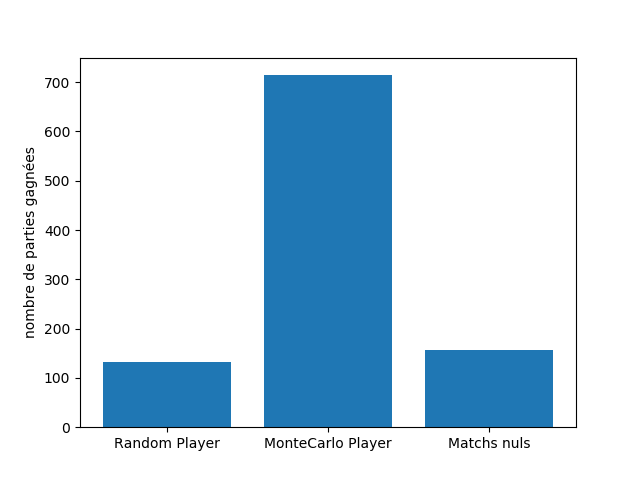
\includegraphics[width=\textwidth]{Report/sections/Figures/Figure16.png}
        \caption{Statistique sur 1000 parties jouées entre un Joueur $Random$ et un Joueur $Monte$ $Carlo$}
    \end{subfigure}
    \begin{subfigure}[b]{0.47\textwidth}
        \centering 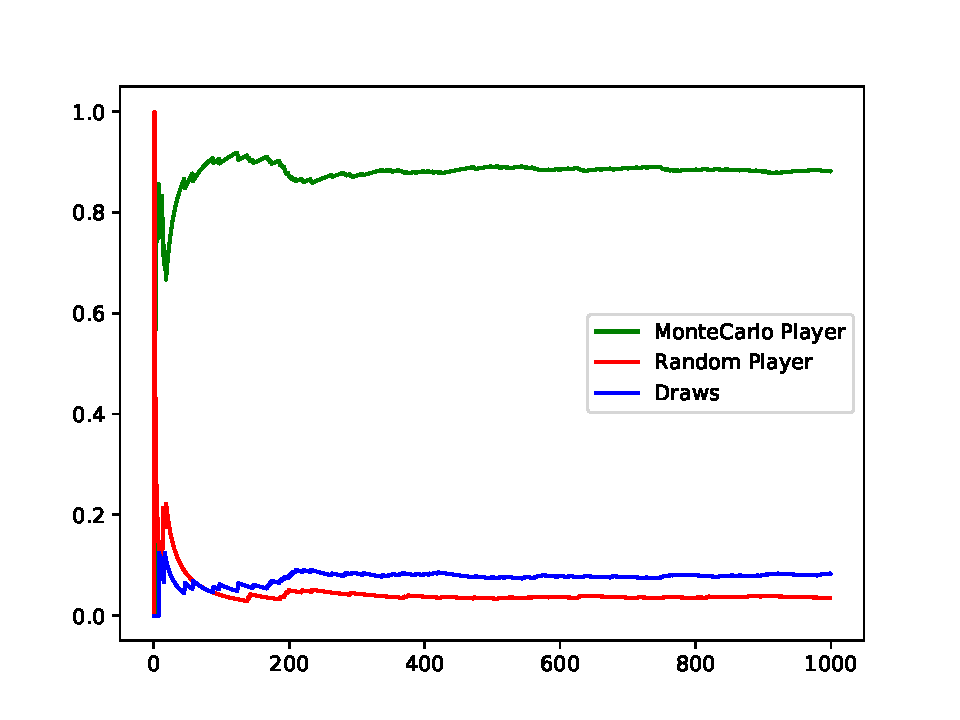
\includegraphics[width=\textwidth]{Report/sections/Figures/Figure17.pdf}
        \caption{Espérance de gain pour chaque joueur}
    \end{subfigure}
    
    \caption{Comparaison entre un Joueur $Random$ et un Joueur $Monte$ $Carlo$}
\end{figure}
\newline
On peut observer sur la figure ci-dessus que le joueur basé sur la méthode de $Monte$ $Carlo$ surpasse largement le joueur $Random$ en terme de parties gagnées. Cependant, il existe des situations où gagner est impossible pour le joueur $Monte$ $Carlo$, malgré le fait que sa politique de jeu soit plus intelligente que celle du joueur $Random$, par exemple, la défaite est inévitable si c'est le joueur $Random$ qui entame la partie et qu'il marque la case centrale en premier, dans ce cas, beaucoup de voies seront bloquées dans la grille et donc peu importe la stratégie du joueur, cela ne lui évitera pas la défaite.
\subsection{Monte Carlo VS Monte Carlo}
\begin{figure}[ht]
\centering
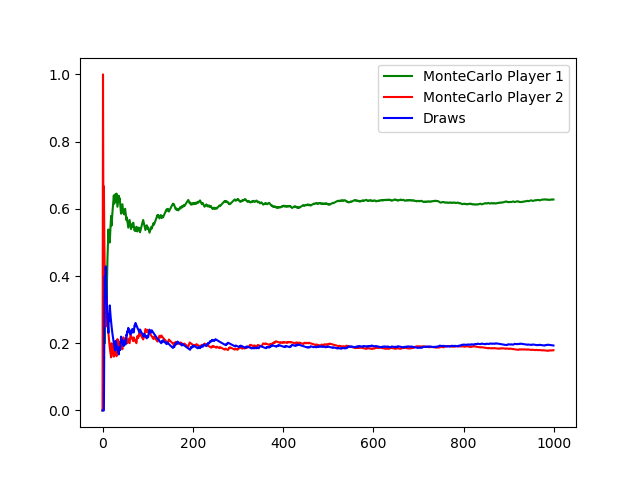
\includegraphics[width=0.6\textwidth]{Report/sections/Figures/Figure13.png}
\caption{Espérance de gain pour deux joueurs $Monte$ $Carlo$}
\label{FigGraphes}
\end{figure}
\newpage
On peur remarquer ici que l'espérance de gain du joueur qui entame la partie est plus elevée que celle du joueur adverse bien qu'ils suivent la meme stratégie de jeu. Cela peut s'expliquer, comme précédemment, par le fait qu'il est presque impossible de gagner pour un joueur lorsqu'il n'entame pas la partie. [à compléter]
\newpage
\part{Monte Carlo Tree Search}
\section{Description de l'algorithme}
L'algorithme Monte Carlo Tree Search est un algorithme de recherche heuristique qui explore intelligemment l'arbre des actions possibles à partir de l'état courant du jeu et ce, jusqu'à ce que toutes les configurations du jeu soient explorées. Cet algorithme choisit en priorité les branches qui sont le plus susceptibles de mener à une victoire. Il maintient par ailleurs un compromis entre l'exploitation et exploration en utilisant l'algorithme UCB pour choisir la prochaine branche à explorer en priorité. 
\section{Implémentation}
Nous avons implémenté cet algorithme à l'aide de trois classes, à savoir \verb@State_Move@, \verb@UCTree@ et \verb@UCTPlayer@. La première représente un couple état-coup, i.e.\ un n\oe ud dans l'arbre de décision. Par ailleurs, \verb@UCTree@ est l'implémentation de cet algorithme à proprement parler car elle contient toutes les fonctionnalités nécessaires à son utilisation. Enfin, \verb@UCPlayer@ correspond au joueur \verb@UCT@. En effet, il hérite de \verb@Agent@ et implémente la méthode \verb@get_action@ dans laquelle il crée un arbre enraciné à l'état courant du jeu et puis, pour $N$ itérations, il simule une partie entre deux joueurs aléatoires et utilise la séquence de coups obtenue pour mettre à jour son arbre de décision en stockant le premier couple état-coup pas encore présent dans l'arbre. La méthode renvoie l'action avec la plus grande récompense.

\section{Mise en oeuvre}
\begin{figure}[!h]
\centering
  \begin{center}
    \subfloat[Espérance de gain contre le joueur $Random$ lorsqu'il entame les parties][Espérance de gain contre le joueur $Random$ lorsqu'il entame les parties]{
      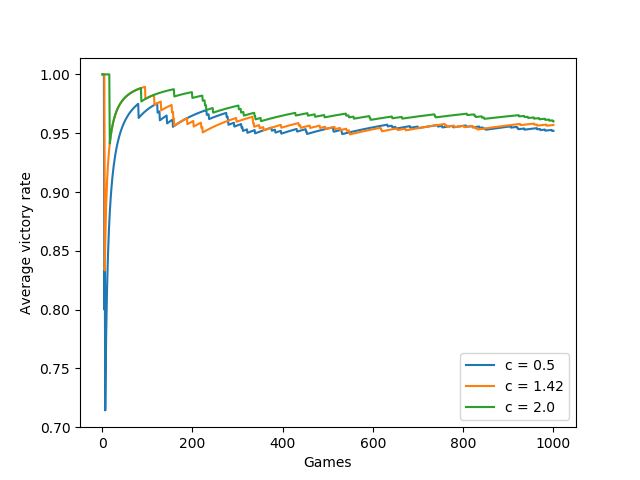
\includegraphics[width=0.5\textwidth]{Project_1/Report/sections/Figures/uct_first_rand.png}
      \label{sub:}
                         }
    \subfloat[Espérance de gain contre le joueur $Random$ lorsque ce dernier entame les parties]{
      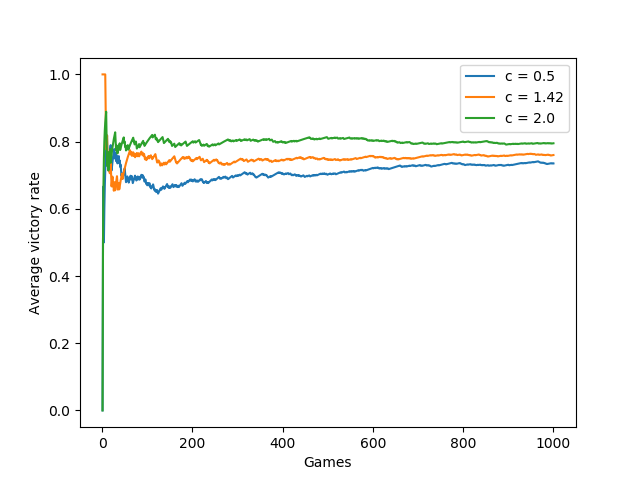
\includegraphics[width=0.5\textwidth]{Project_1/Report/sections/Figures/uct_last_rand.png}
      \label{sub:s}
                          }
    \newline
    \subfloat[Espérance de gain contre le joueur $Monte$ $Carlo$ lorsqu'il entame les parties]{
      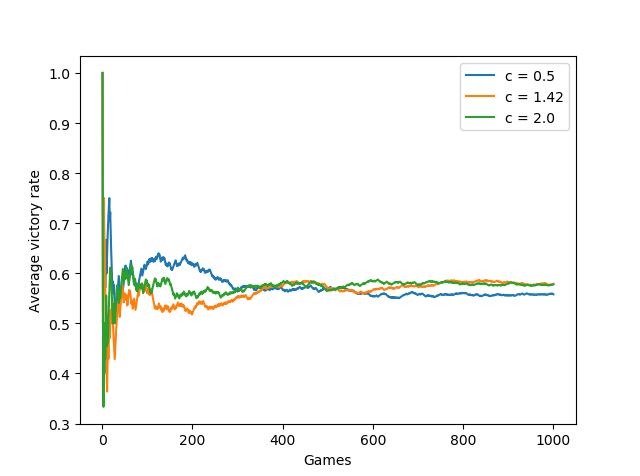
\includegraphics[width=0.5\textwidth]{Project_1/Report/sections/Figures/uct_first_mc.png}      \label{sub:}
                         }
    \subfloat[Espérance de gain contre le joueur $Monte$ $Carlo$ lorsque ce dernier entame les parties]{
      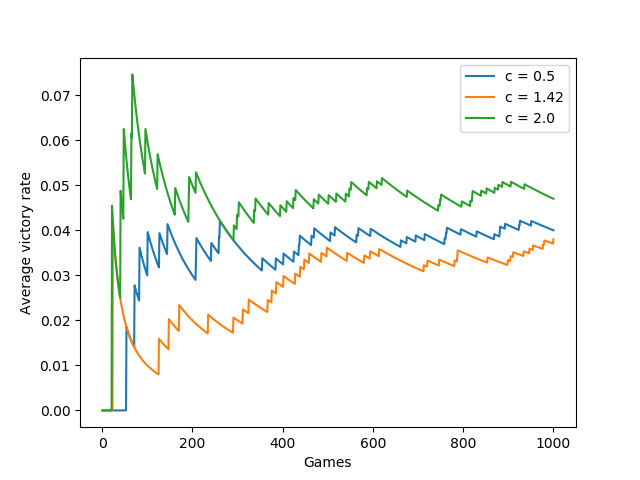
\includegraphics[width=0.5\textwidth]{Project_1/Report/sections/Figures/uct_last_mc.png}
      \label{sub:s}
                          }
    \caption[Benchmark du joueur UCT]{Comparaison entre un joueur $UCT$, avec un nombre d'échantillonnages égal à 100, et les joueurs $Random$ et $Monte$ $Carlo$}
    \label{fig:renonculacees}
  \end{center}
\end{figure}

Dans la figure 7, de la même manière que dans la section 6, le joueur UCT est largement plus intelligent que le joueur aléatoire et ses résultats sont atténués lorsqu'il affronte le joueur Monte Carlo.

Par ailleurs, nous y voyons aussi que la répercussion du paramètre $c$ modulant l'équilibre entre l'exploration et l'exploitation sur les performances de l'algorithme UCT est moindre. En effet, le joueur UCT effectue plus d'exploitation en raison de sa formule qui privilégie les meilleurs coups à différence du joueur $Monte$ $Carlo$ qui explore beaucoup plus de résultats possibles.

C'est ce manque d'exploration qui explique les mauvais résultats du joueur UCT lorsqu'il joue en deuxième vis-à-vis du joueur $Monte$ $Carlo$.
\input{sections/Puissance4.tex}
\newpage
\part*{Conclusion}
\addcontentsline{toc}{part}{Conclusion}
Dans ce projet, nous avons mis en évidence le dilemme de l'exploitation $vs$ exploration à travers divers exemples [à compléter]

% -------------------------------------------------------------------
% Appendices
% -------------------------------------------------------------------

\begin{appendices}
\end{appendices}


\end{document}
